\section{Placement Results}
\label{sec:results}

This section answers the first question in the title. We report the bare-metal
measurement first, because that is where a latency difference can be attributed
to the choice of backup, and then the single-machine runs that corroborate it
over two transports. \S\ref{sec:measurement} takes up the second question: what
had to be controlled for these numbers to mean what they appear to.

\subsection{Bare-Metal Testbed}
\label{sec:testbed}

Eleven bare-metal CloudLab nodes at the Utah cluster
(\texttt{c6525-25g}: one 16-core AMD EPYC 7302P, 128\,GB, 25\,GbE, Ubuntu
22.04). Ten carry the 128 backup servers, thirteen per node except the last;
the eleventh runs the client alone. Each server is launched under
\texttt{taskset} on a core of its own. Hyperthread siblings on this part pair
as $(0,16), (1,17), \dots$, so logical CPUs $2$--$14$ are fourteen distinct
physical cores and no two servers share one core's two threads. The claim that
each backup owned a core is checked rather than asserted: the provisioning tool
records the intended core in a manifest and a verification pass reports the
affinity each server actually holds, together with the ports it answers on. All
replication traffic crosses the 25\,GbE experiment LAN; the control network is
not used for measurement.

Three settings follow from \S\ref{sec:measurement} and are fixed for every run
in this section. Servers listen with a backlog of 512 rather than DEFT's shipped
five, because the shipped value measures connection setup rather than placement
(\S\ref{sec:p99}). Degraded hosts are slowed by \texttt{tc netem} on the
server's own source port rather than by a sleep inside the server, and they are
spread through the host ordering rather than forming a contiguous block
(\S\ref{sec:degconstruct}). One host in eight is degraded at every scale. Each
configuration is 5 context seeds $\times$ 3 trials, giving 15 paired runs of
200 calls per primary at burst 10.

\textbf{What the selectors are told.} The slowdown is physical, but the
knowledge of it is supplied: a degraded host's feature vector carries the
degraded health and capacity values of \S\ref{sec:methods}. These runs therefore
measure what it costs to select a degraded host and what is gained by avoiding
one, \emph{given accurate host state}. Whether a scoring function can recognise
degradation from realistic, partial signals is a separate question, which
\S\ref{sec:weights} answers.

\subsection{Heterogeneous Pools: Feature-Aware Selection Avoids Degraded Hosts}
\label{sec:hetero}

% Generated by make_testbed_tables.py -- do not edit by hand.
\begin{table}[t]
\centering
\caption{Mean service latency and the share of calls reaching a degraded backup, at three scales on the same bare-metal testbed. Every backup is pinned to its own physical core and the degraded hosts are slowed by \texttt{tc netem} on the server's source port. 12.5\% of hosts are degraded at every scale. Milliseconds.}
\label{tab:scales}
\resizebox{\columnwidth}{!}{%
\begin{tabular}{lrrrrrr}
\toprule
& \multicolumn{2}{c}{16 hosts} & \multicolumn{2}{c}{32 hosts} & \multicolumn{2}{c}{128 hosts} \\
\cmidrule(lr){2-3}\cmidrule(lr){4-5}\cmidrule(lr){6-7}
Method & Mean & Degr.\% & Mean & Degr.\% & Mean & Degr.\% \\
\midrule
\texttt{exact} & 23.17 & 0.00 & 31.27 & 0.00 & 41.76 & 0.00 \\
\texttt{heuristic} & 23.82 & 0.00 & 31.59 & 0.00 & 42.03 & 0.00 \\
\texttt{round\_robin} & 29.89 & 10.00 & 38.65 & 10.00 & 51.87 & 12.50 \\
\texttt{random} & 36.45 & 18.00 & 40.88 & 15.00 & 51.25 & 11.25 \\
\texttt{PPO} & 23.49 & 0.00 & 32.37 & 1.00 & 45.04 & 0.00 \\
\texttt{concentrated} & 101.71 & 100.00 & 98.35 & 95.00 & 260.11 & 100.00 \\
\bottomrule
\end{tabular}}
\end{table}


Table~\ref{tab:scales} reports all three scales. The mechanism is in the
right-hand column of each pair. \texttt{heuristic} and \texttt{optimal} route a
primary to a degraded backup in $0.00\%$ of calls at 16, 32 and 128 hosts.
\texttt{round\_robin} meets degraded hosts at $10.00$--$12.50\%$, the base rate,
and \texttt{random} at $11.25$--$18.00\%$.

The latency follows the selection. The better feature-aware method beats
\texttt{round\_robin} by $6.72$\,ms at 16 hosts, $7.38$ at 32 and $10.11$ at
128, about a fifth of the mean at every scale, and roughly halves p99: $49$
against $121$\,ms, $68$ against $137$, and $80$ against $157$. The paired
comparisons of \texttt{optimal} against \texttt{round\_robin} have $r = -1.000$
at all three scales, meaning no run dissents, and against \texttt{random}
$r \le -0.967$ (all $p_{\mathrm{Holm}} \le 0.0011$). The gap widens with the
pool, as expected when blind selection has more degraded hosts to meet.

\textbf{The greedy heuristic matches the exact assignment.} \texttt{heuristic}
versus \texttt{optimal} is not significant at any scale
($p_{\mathrm{Holm}} \ge 0.62$ on the mean; $1.000$ on p99 at 128 hosts). The
exact solve is therefore a useful bound rather than a necessary deployment.

\textbf{What $0\%$ does and does not mean.} The zero is a statement about
selection under accurately reported host state, with a fixed set of impaired
hosts. An orchestrator's telemetry is noisier and arrives late, and under it a
feature-aware selector will sometimes choose a host that has just degraded. The
comparison that carries over is the relative one: a selector that reads host
state avoids degraded hosts to the extent the state is right, and an order-based
one meets them at the base rate regardless.

\textbf{The concentrated arm.} With degraded hosts spread through the ordering,
the host \texttt{concentrated} piles onto is itself degraded, so its figures
here conflate concentration with degradation. The clean figure for concentration
alone is the homogeneous one below.

\subsection{Homogeneous Pools: Selection Does Not Matter}
\label{sec:homog}

With all 128 hosts identical and none degraded, \texttt{optimal},
\texttt{heuristic}, \texttt{round\_robin} and \texttt{random} are statistically
indistinguishable at $41.5$--$42.0$\,ms mean. The paired comparison of
\texttt{optimal} against \texttt{random} gives a median difference of
$0.002$\,ms ($p_{\mathrm{Holm}} = 1.000$). Only \texttt{concentrated}
($56.27$\,ms, $35\%$ above \texttt{optimal}) and the learned policy
($46.53$\,ms) separate from the group.

This bounds the claim. Where every candidate is equivalent, a selector that
reads node features has nothing to read, and the exact assignment buys nothing
over choosing uniformly at random. What still matters is not piling every
primary onto one backup. The result also serves as the negative control for the
previous subsection: the apparatus does not manufacture an advantage for
feature-aware methods where none should exist.

\subsection{Corroboration on One Machine, over Two Transports}
\label{sec:scale32}

\begin{table}[t]
\centering
\caption{Per-call service latency by topology scale and transport. XML-RPC: 15
runs; gRPC: 25 runs (5 context seeds $\times$ 5 trials), 200 calls/primary,
burst 10. Effect sizes are paired against \texttt{heuristic} on the gRPC arm.
\texttt{baseline} is DEFT's shipped static mapping, which exists only for the
9-host topology. The 9-host scenario is homogeneous and serves as the negative
control: with nothing to discriminate between candidates, every method except
\texttt{concentrated} and \texttt{baseline} is indistinguishable from the
heuristic.}
\label{tab:scalesweep}
\resizebox{\columnwidth}{!}{%
\begin{tabular}{llrrrrr}
\toprule
& & XML-RPC & \multicolumn{4}{c}{gRPC} \\
\cmidrule(lr){3-3}\cmidrule(lr){4-7}
Scale & Method & Mean (ms) & Mean (ms) & 95\% CI & $r$ & $p_{\mathrm{Holm}}$ \\
\midrule
\multirow{7}{*}{\shortstack[l]{9 hosts\\5 primaries\\homogeneous}}
 & \texttt{baseline} & 73.45 & 20.58 & [17.55, 24.56] & $+0.680$ & 0.0243 \\
 & \texttt{concentrated} & 107.42 & 32.60 & [29.84, 35.77] & $+1.000$ & $<$0.0001 \\
 & \texttt{random} & 58.70 & 16.04 & [14.50, 17.75] & $+0.329$ & 0.7817 \\
 & \texttt{round\_robin} & 47.51 & 14.06 & [12.22, 16.43] & $-0.422$ & 0.5010 \\
 & \texttt{heuristic} & 51.10 & 14.72 & [13.44, 16.18] & -- & -- \\
 & \texttt{optimal} & 45.90 & 13.60 & [12.50, 14.92] & $-0.286$ & 0.8799 \\
 & \texttt{PPO} & 48.44 & 13.79 & [12.06, 16.21] & $-0.403$ & 0.5010 \\
\midrule
\multirow{6}{*}{\shortstack[l]{16 hosts\\10 primaries\\2 degraded}}
 & \texttt{concentrated} & 175.36 & 77.97 & [72.12, 83.99] & $+1.000$ & $<$0.0001 \\
 & \texttt{random} & 145.00 & 31.45 & [24.34, 39.47] & $+0.655$ & 0.0185 \\
 & \texttt{round\_robin} & 144.21 & 26.23 & [24.08, 29.12] & $+0.705$ & 0.0104 \\
 & \texttt{heuristic} & 98.35 & 17.88 & [14.03, 22.76] & -- & -- \\
 & \texttt{optimal} & 90.73 & 18.82 & [14.30, 24.45] & $-0.046$ & 1.0000 \\
 & \texttt{PPO} & 89.38 & 13.83 & [12.57, 15.49] & $-0.200$ & 1.0000 \\
\midrule
\multirow{6}{*}{\shortstack[l]{32 hosts\\20 primaries\\4 degraded}}
 & \texttt{concentrated} & 296.00 & 121.13 & [116.06, 127.00] & $+1.000$ & $<$0.0001 \\
 & \texttt{random} & 172.59 & 31.84 & [23.14, 43.35] & $+0.945$ & $<$0.0001 \\
 & \texttt{round\_robin} & 163.39 & 28.62 & [22.64, 39.73] & $+0.994$ & $<$0.0001 \\
 & \texttt{heuristic} & 121.39 & 13.25 & [12.15, 14.95] & -- & -- \\
 & \texttt{optimal} & 123.29 & 19.15 & [12.49, 30.49] & $-0.022$ & 1.0000 \\
 & \texttt{PPO} & 130.38 & 13.22 & [12.34, 14.33] & $+0.126$ & 1.0000 \\
\bottomrule
\end{tabular}}
\end{table}

The same comparison was first run with every host as a process on one machine,
over both transports (Table~\ref{tab:scalesweep}, Fig.~\ref{fig:latencyscale}).
We keep these runs for two reasons. They show the finding does not depend on one
RPC stack, and they are the data in which the measurement effects of
\S\ref{sec:measurement} were found. Their absolute latencies carry three
caveats: the hosts share one machine, the XML-RPC arm uses the shipped backlog,
and differences below the $10$\,ms resolution floor of \S\ref{sec:stats} are
not claimed.

\textbf{9 hosts, homogeneous.} This scenario was not re-run on bare metal and
serves as a negative control only. \texttt{round\_robin}, \texttt{optimal}, the
learned policy and \texttt{random} are indistinguishable from the heuristic on
both transports, and the two transports agree on that null to within
$0.06$\,ms. We draw no conclusion from its absolute latencies.

\textbf{16 and 32 hosts, heterogeneous.} \texttt{heuristic}, \texttt{optimal}
and the learned policy never route a primary to a degraded host in any seed.
\texttt{round\_robin} hits one on 2 of 10 and 4 of 20 assignments in every seed,
and \texttt{random} between none and four depending on the seed. On the gRPC arm
at 32 hosts the heuristic beats \texttt{round\_robin} by $9.75$\,ms at the median
run ($r=0.994$, $p_{\mathrm{Holm}}<0.0001$) and \texttt{random} by $13.10$\,ms
($r=0.945$). At 16 hosts the same comparisons give $r=0.705$
($p_{\mathrm{Holm}}=0.0104$) and $r=0.655$ ($p=0.0185$). \texttt{optimal} and
the learned policy are indistinguishable from the heuristic at both scales
($|r| \le 0.20$, all $p_{\mathrm{Holm}} = 1.000$).

The ordering therefore agrees with the bare-metal runs on both transports. The
magnitudes do not, and should not be read as placement effects: on this harness
the same comparison appears worth a third to a half of the mean, against a
fifth on bare metal, for the reasons \S\ref{sec:p99} gives. One row is also
specific to how these runs were built. The degraded hosts here are the first
$n$ of the backup-eligible set, so the host \texttt{concentrated} piles onto
happens to be healthy; \S\ref{sec:degconstruct} explains why that construction
cannot be trusted.

\begin{figure}[t]
\centering
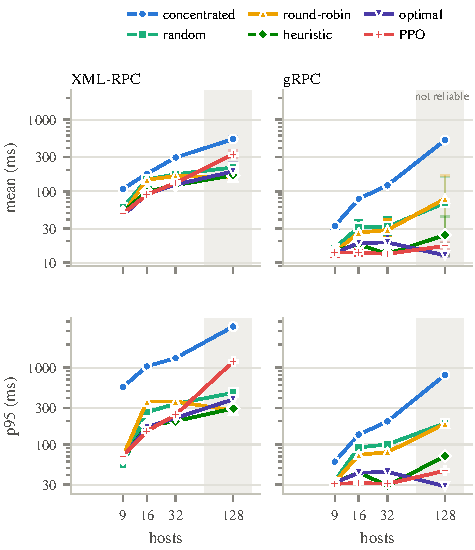
\includegraphics[width=\columnwidth]{figures/fig_latency_scale.pdf}
\caption{Per-call service latency vs.\ topology scale, by transport (log axes).
Top row: mean with cluster-bootstrap 95\% confidence intervals. Bottom row: p95.
The 9-host point is the homogeneous scenario (its \texttt{baseline} method, which
exists only there, is omitted). The p95 row shows the degraded-host penalty
\texttt{round\_robin} and \texttt{random} pay at 16 and 32 hosts, which the gRPC
arm separates more cleanly because its baseline latencies are an order of
magnitude lower. The 128-host column is shaded and its confidence
intervals are drawn faded: independent executions of that configuration differ
several-fold on either transport, so it is not a usable latency measurement on
a single machine (\S\ref{sec:single128}).}
\label{fig:latencyscale}
\end{figure}

\subsection{Mechanism: Latency Follows Backup Load}
\label{sec:backupload}

Table~\ref{tab:backupload} pools service latency by the number of primaries
sharing a backup, aggregated to one observation per (run $\times$ backup) so
that correlated calls against one loaded server count once. Mean latency rises
monotonically with load, whichever method produced the sharing. This is what
licenses scoring a mapping \emph{structurally}, by how many distinct backups it
uses and its peak load, where latency cannot be measured.

\begin{table}[t]
\centering
\caption{Service latency vs.\ backup load on the XML-RPC arm, one observation per (run $\times$ backup).}
\label{tab:backupload}
\resizebox{\columnwidth}{!}{%
\begin{tabular}{clrrr}
\toprule
Scenario & Load & $n$ units & Mean (ms) & 95\% CI \\
\midrule
\multirow{4}{*}{Homog.} & 1 & 354 & 45.23 & [44.60, 45.89] \\
 & 2 & 33 & 68.07 & [65.80, 70.35] \\
 & 3 & 15 & 96.94 & [90.51, 104.25] \\
 & 4 & 15 & 126.20 & [117.85, 135.44] \\
\midrule
\multirow{4}{*}{16-host} & 1 & 678 & 104.56 & [98.86, 110.46] \\
 & 2 & 21 & 107.14 & [100.41, 113.65] \\
 & 3 & 15 & 229.03 & [115.11, 349.47] \\
 & 9 & 15 & 190.79 & [181.37, 199.20] \\
\bottomrule
\end{tabular}}
\end{table}

\subsection{Decentralized Baselines and Topology Diversity}
\label{sec:hrw}

Replica placement is well studied where storage is the subject, so we add the
baselines that literature would expect: rendezvous hashing, health- and
capacity-weighted rendezvous hashing, and Dynamo-style weighted consistent
hashing~\cite{weil2006crush,decandia2007dynamo}, scored structurally
(Table~\ref{tab:hrw}).

Plain rendezvous hashing is quality-unaware and its degraded-host exposure is
correspondingly uncontrolled. Both weighted variants avoid degraded hosts
entirely at every scale, which establishes that \emph{quality-awareness, not
centralization, is what buys avoidance}. They are coordination-free, however ---
each primary hashes independently with no load penalty propagated --- so they
spread load only statistically: mean peak per-backup load is $3.0/3.6/2.2$ and
$2.8/3.0/3.2$ at 16/32/128 hosts, against the greedy heuristic's $1.4/2.0/2.0$
and the exact assignment's $1.0$. A single coordinated pass load-balances
materially tighter than either weighted-hash family at equal avoidance.

Two robustness checks accompany this. A randomized-offset round-robin removes
the naming dependence examined in \S\ref{sec:degconstruct}, and then meets degraded
hosts at every scale in proportion to the degraded fraction. And repeating the
comparison on multi-hub topologies, where host-to-host hop count and latency
vary, leaves the structural outcome unchanged: avoidance and load balancing are
driven by host quality rather than graph shape.

\begin{table}[t]
\centering
\caption{Decentralized hash baselines and a fairer round-robin vs.\ the feature-aware
methods, 5-seed average, heterogeneous star scenarios (multi-hub results are identical; see
text). ``Deg.'' = mean primaries routed to a degraded host (lower is better); ``Load'' = mean
max per-backup load (lower is a tighter spread).}
\label{tab:hrw}
\resizebox{\columnwidth}{!}{%
\begin{tabular}{lcccccc}
\toprule
& \multicolumn{2}{c}{16-host} & \multicolumn{2}{c}{32-host} & \multicolumn{2}{c}{128-host}\\
\cmidrule(lr){2-3}\cmidrule(lr){4-5}\cmidrule(lr){6-7}
Method & Deg. & Load & Deg. & Load & Deg. & Load \\
\midrule
round\_robin & 2.0 & 1.0 & 4.0 & 1.0 & 0.0 & 1.0 \\
rr\_random & 1.2 & 1.0 & 2.6 & 1.0 & 10.8 & 1.0 \\
hrw & 2.0 & 3.0 & 0.0 & 3.0 & 9.0 & 2.0 \\
weighted\_hrw & 0.0 & 3.0 & 0.0 & 3.6 & 0.0 & 2.2 \\
weighted\_chash & 0.0 & 2.8 & 0.0 & 3.0 & 0.0 & 3.2 \\
heuristic & \textbf{0.0} & \textbf{1.4} & \textbf{0.0} & \textbf{2.0} & \textbf{0.0} & \textbf{2.0} \\
optimal & 0.0 & 1.0 & 0.0 & 1.0 & 0.0 & 1.0 \\
\bottomrule
\end{tabular}}
\end{table}

\subsection{The Learned Policy as a Secondary Baseline}
\label{sec:rl128}
\label{sec:dqn}

We include a learned policy because reinforcement learning is the usual
proposal for NFV placement (\S\ref{sec:related}), not because the comparison is
symmetric. The heuristic needs no training. The policy needs a model per host
count and tuning that grows with scale. We therefore state the tuning it
received and keep the claim narrow.

\textbf{Tuning effort.} Both learners were given comparable budgets, and we
state them so the comparison can be judged. Through 32 hosts each was trained
once per scale on a single configuration: a $[128,128]$ network for both, with
entropy $0.01$ for PPO and $\epsilon$-greedy decay over the first $30\%$ of
training for DQN, at 50k, 80k and 100k timesteps. These are our defaults, not
the library's, which are smaller on both counts. Two scales then needed more.
DQN at 32 hosts collapsed onto 2--4 of 20 backups under that configuration, a
figure we measured directly from the released checkpoint rather than inferred.
It was retrained with exploration widened to $70\%$ of training, a final
$\epsilon$ of $0.15$, a doubled replay buffer and 150k timesteps, which lifted
it to 12--16 and is the checkpoint Table~\ref{tab:ppodqn} reports. At 128 hosts PPO was trained three times: once at the library
defaults ($[64,64]$, entropy $0$, 400k steps), which collapsed onto 1--5
backups; once at $[128,128]$ with entropy $0.01$ and 600k steps, which improved
only partly and is not released; and once at $[256,256]$ with entropy $0.02$,
larger rollouts and 1M timesteps, which is the configuration reported. DQN at
128 hosts received the matching $[256,256]$ network, a widened exploration
schedule and the same 1M timesteps. Counting training runs, PPO received six
and DQN five, with DQN given the larger budget at the one scale where both were
retuned. This is a targeted search rather than an exhaustive one, and a larger
budget might do better for either.

\textbf{Result.} The policy avoids degraded hosts as well as the deterministic
methods: $0\%$ of calls at 16 and 128 hosts and $1\%$ at 32
(Table~\ref{tab:scales}). It is indistinguishable from \texttt{optimal} at 16
and 32 hosts and significantly slower at 128
($p_{\mathrm{Holm}} = 0.0009$, $r = -0.983$). Its structure explains the gap.
In the 128-host runs it placed its 80 primaries on 15--18 distinct backups per
run, against the heuristic's 72--78 and the exact assignment's 80. It learned
which hosts are bad, but not to spread load.

\begin{table}[t]
\centering
\caption{PPO vs.\ DQN policy structure, 5 context seeds per scale. ``Distinct'' is the range
of distinct backups a policy assigns its primaries across seeds (higher is a wider spread),
``Peak'' the largest number of primaries placed on any one backup (lower is better), and
``Degraded'' the assignments landing on a deliberately degraded host, out of 5 seeds
$\times$ $|P|$.}
\label{tab:ppodqn}
\resizebox{\columnwidth}{!}{%
\begin{tabular}{llrrr}
\toprule
Scale & Algorithm & Distinct & Peak & Degraded \\
\midrule
\multirow{2}{*}{9-host} & PPO & 5--5 of 5 & 1--1 & 0/25 \\
 & DQN & 5--5 of 5 & 1--1 & 0/25 \\
\midrule
\multirow{2}{*}{16-host} & PPO & 10--10 of 10 & 1--1 & 0/50 \\
 & DQN & 9--10 of 10 & 1--2 & 0/50 \\
\midrule
\multirow{2}{*}{32-host} & PPO & 15--19 of 20 & 2--2 & 0/100 \\
 & DQN & 12--16 of 20 & 2--3 & 1/100 \\
\midrule
\multirow{2}{*}{128-host} & PPO & 24--30 of 80 & 9--28 & 0/400 \\
 & DQN & \textbf{1--3 of 80} & \textbf{45--80} & \textbf{172/400} \\
\bottomrule
\end{tabular}}
\end{table}

\textbf{A second algorithm fails the same way.} We trained a DQN
agent~\cite{mnih2015human} through the same environment, reward and inference
path, and scored both structurally (Table~\ref{tab:ppodqn}). The two agree
through 32 hosts. At 128 hosts DQN collapses onto 1--3 of 80 backups, with 172
of 400 assignments on degraded hosts. An ablation of the reward's
anti-concentration term, released with the artifact, shows the term helps but
saturates well short of the heuristic's spread. Two algorithms with different
update rules and exploration mechanisms failing alike points at the reward,
which credits concentration at the step where it occurs while the consequences
accrue later, rather than at either learner.

\textbf{What we claim.} For this problem a deterministic heuristic already
matches the exact assignment, so a learned policy has no headroom to win, and it
adds a per-scale training and tuning burden. We do not claim that RL cannot be
made to work at 128 hosts.

\subsection{Selection Overhead and Throughput}
\label{sec:overhead}
\label{sec:throughput}

Selection must itself be fast. Table~\ref{tab:overhead} reports mean wall-clock
time per full mapping (30 repeats, first call excluded). Every non-learned
method computes a 128-host mapping in roughly $10$\,ms or less and the learned
policy in about $60$\,ms, against failure-detection intervals of hundreds of
milliseconds to seconds~\cite{gill2011understanding,potharaju2013demystifying}.
No method's selection cost offsets its placement advantage.

Fixed-window throughput and post-retry failure rate agree with latency where
they resolve. \texttt{concentrated} is robustly worst on both
($r \in [0.63, 0.78]$, every $p < 0.004$; failure rate $2.57\%$ against
$0.16$--$0.62\%$). The remaining methods do not separate at 15 aggregate
measurements each, which we read as a limit of that measurement, so the
comparison rests on latency.

\begin{table}[t]
\centering
\caption{Selection overhead (ms) per full mapping computation, mean of 30 repeats
(first call excluded as warmup).}
\label{tab:overhead}
\resizebox{\columnwidth}{!}{%
\begin{tabular}{lrrrr}
\toprule
Method & 9 hosts & 16 hosts & 32 hosts & 128 hosts \\
\midrule
\texttt{concentrated} & 0.006 & 0.021 & 0.035 & 0.600 \\
\texttt{random} & 0.028 & 0.043 & 0.054 & 0.567 \\
\texttt{round\_robin} & 0.005 & 0.007 & 0.009 & 0.055 \\
\texttt{heuristic} & 0.050 & 0.145 & 0.600 & 10.277 \\
\texttt{optimal} & 0.081 & 0.271 & 0.860 & 9.968 \\
\texttt{PPO} & 6.345 & 5.065 & 10.605 & 61.636 \\
\texttt{DQN} & 1.404 & 6.209 & 6.217 & 40.080 \\
\bottomrule
\end{tabular}}
\end{table}
